% !TEX encoding = UTF-8 Unicode
%!TEX root = main.tex
% !TEX spellcheck = en-US
%%=========================================

\chapter{Design}
\label{ch:design}

This chapter explains in detail the design behind the core elements in ProXC. First the foundation of the run\hyp{}time system is explained, and how processes and the scheduler coordinate in this environment. The design of composite process creation and execution is explained, and how this works in the process and scheduler coordination. Further on, the more abstract constructs channels, timers, and alternation are detailed. And lastly, the design of the API for the library is described, and what influences has driven the design. 


\section{Run\hyp{}time System}
\label{sec:runtime_system}

The run\hyp{}time system of ProXC forms the foundation for how the library is able to implement a CSP model in C. Some sort of a threading model has to be implemented when implementing a CSP model for programming, which is discussed in Section \ref{sec:concurrency_vs_parallelism}, \ref{sec:threading_models} and \ref{sec:csp}. The choice of threading model is an important choice regarding performance, and is analysed in \citet[chapter 1]{c++csp2}. The paper reasons that the context switch time between threads is the major factor in performance, and argues that the hybrid model would be the best choice for the CSP library. This is reasoned from the added flexibility and benefits of using the combination of user\hyp{}threads and kernel\hyp{}threads, allowing fast user\hyp{}threads for tightly coupled processes, and kernel\hyp{}threads on looser couplings across thread boundaries. Based on this, a hybrid threading model is used for ProXC. 

The core of the run\hyp{}time system is the scheduler, which controls the flow of execution of processes. In the threading model, each kernel\hyp{}thread has a permanent corresponding scheduler, scheduling multiple processes on said kernel\hyp{}thread. However, it is important to understand that the scheduler itself is a user\hyp{}thread on the kernel\hyp{}thread. Each process is a user\hyp{}thread. The kernel\hyp{}thread executes only one user\hyp{}thread at the time, and the scheduler decides which process is to be resumed by context switching. The context switch only switches between the scheduler and a process context, or vice versa. 

\begin{figure}[h]
    \centering
    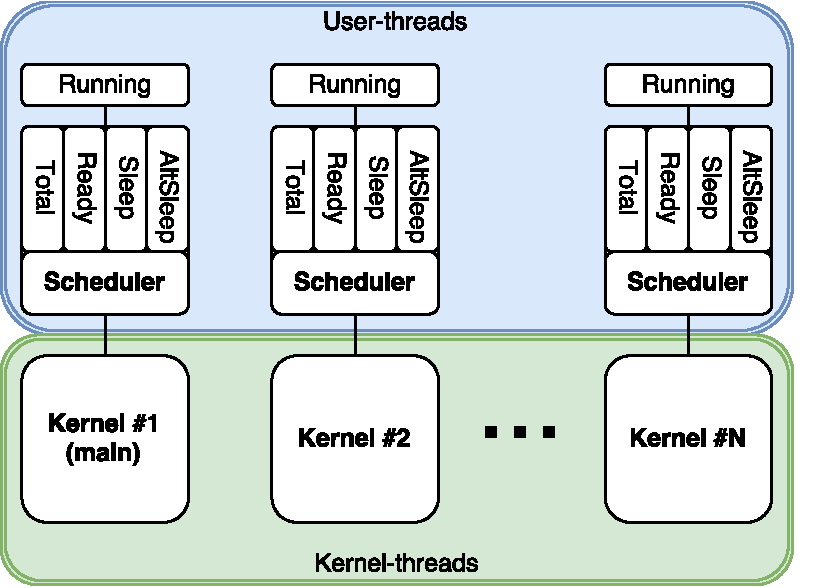
\includegraphics[width=0.6\linewidth]{fig/run-time_system}
    \caption{Overview of the run-time system, with N online processor cores}
    \label{fig:run-time_system}
\end{figure}

The run\hyp{}time system at start up spawns a number of kernel\hyp{}threads equal to the number of online processor cores minus 1. This comes from that the main thread is running on its own kernel\hyp{}thread, which the run\hyp{}system hijacks. This kernel\hyp{}thread is marked as the main kernel\hyp{}thread. When the scheduler on the main kernel\hyp{}thread is exited, the run\hyp{}time system is signaled to cleanup and exit. The run\hyp{}time system initializes the thread\hyp{}specific data key, which is used by the library to find out which scheduler corresponds to which kernel\hyp{}thread. This is explained in more detail in Section \ref{sec:thread_specific_data}.

\subsection*{Terminology}

From here on, the term ``\textit{process}'' means a single user\hyp{}thread meant to run sequential code from a program. The term ``\textit{parent scheduler}'' in the context of a process means the scheduler which the process is designated to, i.e. both reside on the same kernel\hyp{}thread. The term ``\textit{running process}'' corresponds to the process that is currently executed on a given kernel\hyp{}thread, given that the scheduler has resumed a process. The term ``\textit{ownership}'' in the context of a scheduler owning a process means the scheduler is a parent scheduler to the process. The term ``root process'' in the context of composite processes means the process that defined and spawned the composite process.

\subsection{Scheduler}
\label{sec:scheduler}

The scheduler keeps track of the execution state of a kernel\hyp{}thread. Each scheduler knows which process is the main process, as this is important later. As well, it keeps track of the current process running. 

\subsubsection*{Execution Context}

As mentioned above, the scheduler runs in its own user\hyp{}thread. It is however important to state that the scheduler does not need to allocate a stack for its user\hyp{}thread, as it uses the user stack in the kernel\hyp{}thread as its own local stack. This is not the case for processes, which is explained in Section \ref{subsec:processes}.

\subsubsection*{Data Structures}

A couple of data structures are used in the scheduler. It has two queues: a ready queue and a total queue. It also has two trees: a sleep tree and a alternating guard sleep tree. The ready queue is a queue of processes that are ready to be executed. The total queue is the total collection of all processes that are present in the scheduler. The sleep tree is a minimal ordered tree of sleeping processes, where the root node of the tree is the process with the smallest time left sleeping. The alternation guard sleep tree is the same as the sleep tree, where it contains alternation guards instead of processes.

\subsubsection*{Scheduler Phases}

The schedulers main loop has three phases: prologue, context switch, and epilogue. Each phase corresponds to what it does before, under and after a context switch to a process. 

In prologue the scheduler does a termination test, checks if any processes are available, wakes up any timed out processes, and finds next process to resume. The termination test succeeds if either the total queue is empty, or the exit flag is set. Checking the ready queue ensures there are any processes available, and if not, suspends the kernel\hyp{}thread until either a process becomes ready. A process becomes ready by either timing out in the sleep trees, or is added to the ready queue by an another scheduler. When a process is ready, the scheduler checks the sleep trees and adds any processes that has timed out to the ready queue. Lastly, it finds which process from the ready queue to resume.

After prologue, the scheduler now has a process to resume execution to. First, the process is registered as the running process in the scheduler. This is important for later, explained in Section \ref{sec:thread_specific_data}. Then, the actual context switch to the process happens. From here, the flow of execution in the kernel\hyp{}thread jumps from the scheduler to the context of the process. Whenever the process is descheduled, either through an implicit or explicit descheduling point, the flow of execution is returned to the scheduler, and it resumes as if the function call returned. When returned, the scheduler advises the kernel on the memory of the process stack it is not using. This allows the kernel to reduce the actual memory footprint of the run\hyp{}time system.

In epilogue, the state of the returned process is checked and appropriately handled. Currently only the return states of an unaltered process state or an ended process state is handled. The process is added back to the ready queue, or the process is cleaned up, respectively. If the ended process is the main process, the exit flag in the scheduler is set. Lastly, the running process information is reset in the scheduler, and loops back to prologue.

In Listing \ref{lst:scheduler_main_loop}  is the pseudo code of the following phases shown.
\begin{lstlisting}[style=CustomC,caption={Pseudo code for scheduler main loop},label={lst:scheduler_main_loop}]
void scheduler() {
    // Phase 1: Prologue
    while ( termination_test() ) {
        wait_for_readyQ_if_empty();
        check_timedout_processes();
        current_proc = find_next_process();
        
        // Phase 2: Context switch
        register_running_proc(current_proc);
        context_switch(current_proc);
        advise_memory(current_proc.stack);
        
        // Phase 3: Epilogue
        check_state(current_proc);
        reset_running_proc();      
    }
    // Here the scheduler exits, and the run-time takes over
}
\end{lstlisting}

It is important to note that when entering phase 3, the state of the returned process is chan\-ged in the context of the process. So even though the scheduler sets the state of the process to running in phase 1, the process state can and will be changed when execution is returned to the scheduler. This is of course done by the library, and is invisible to the programmer.


\subsection{Processes}
\label{subsec:processes}

A process is a sequential execution of code. In ProXC, and consequently in C, the sequential code is written as a normal function. The process keeps track of which function to execute and its arguments, the context of the function, the stack of which the context is executed in, and the state of the process. The process does also express some notion of ownership, as it acknowledges the parent scheduler is the only scheduler it assigns to.

\subsubsection*{Execution Context}

The processes and the scheduler are both executed as user\hyp{}threads. This means each user\hyp{}thread has its own stack and context. However, as opposed to the scheduler, processes has to allocate its own stack. This is done by the run\hyp{}time system.

\subsubsection*{Process States}

The process state describes the current state of the process. In the run\hyp{}time system, the process state is used for a couple of things: informing the scheduler the reason for why the process returned control, knowing when the process ended, and separating the processes in the correct FIXME. The complete finite state machine of all possible process states and transitions are shown in Figure \ref{fig:process_state_fsm}. 
 
\FloatBarrier

\begin{figure}[h]
    \centering
    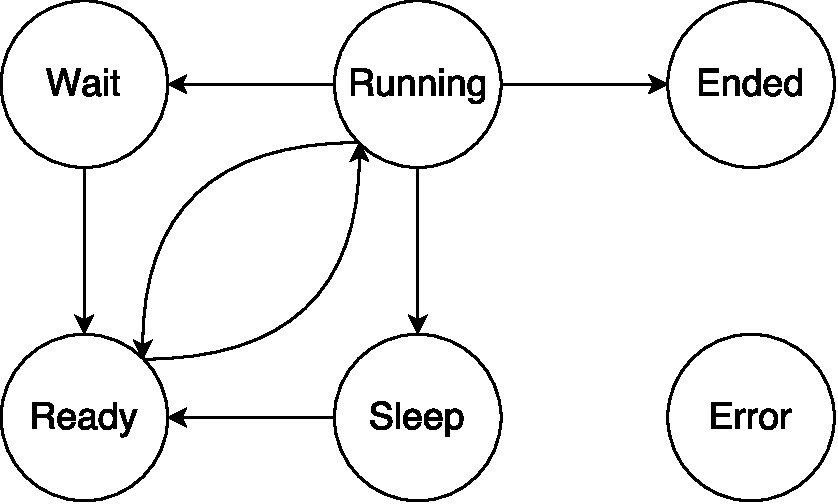
\includegraphics[width=0.6\linewidth]{fig/process_state_fsm}
    \caption{finite state machine of process states and transitions}
    \label{fig:process_state_fsm}
\end{figure}

\FloatBarrier

The process states describes the following: 
\begin{itemize}
    \setlength\itemsep{0em}
    \item \textbf{Ready state}: the process is in a scheduler's ready queue and is ready to be resumed. 
    \item \textbf{Running state}: the process is currently being executed on a kernel\hyp{}thread, and the\\ scheduler is waiting for the process to return control.
    \item \textbf{Ended state}: the process has reached the end of its sequential code, and can safely\\ be cleaned up.
    \item \textbf{Error state}: the process has entered an unrecoverable state.
    \item \textbf{Wait state}: the process is waiting for an another process to release it. This can happen during synchronization points such as channel communication and alternation without timeout.
    \item \textbf{Sleep state}: the process is suspended for a given amount of time, and is waiting for time out. This happens during explicit suspension or alternation with timeout.  
\end{itemize}

A couple constraints regarding the process states and transitions needs to be addressed. When a process is created, the process state is initially set to \textit{Ready}. Only the parent scheduler can transition the process state from \textit{Ready} to \textit{Running}. This transition transfers the flow of control from the parent scheduler to the running process. Only one process can be in the \textit{Running} state at the time on a given scheduler. This should be logical, given that only one user\hyp{}thread is able to be executed at a time on a kernel\hyp{}thread. The transition from \textit{Running} to either \textit{Ready}, \textit{Ended}, \textit{Wait} or \textit{Sleep} can only be done be the running process itself. This transition also follows that the flow of control is transferred back to the parent scheduler. The transition from \textit{Wait} or \textit{Sleep} to \textit{Ready} is either done by the parent scheduler or by other running processes. The transition to \textit{Error} can happen from anywhere at any time, and is used by the run\hyp{}time system to detect unrecoverable process states.


\subsection{Scheduler and Process Interaction}
\label{subsec:scheduler_process_interaction}

This has been briefly mentioned in the preceding subsections, but should be more accurately defined. Processes and schedulers are not entirely isolated, and interactions are frequent between them.

The scheduler manipulates the process states directly, in the transitions from \textit{Ready} to \textit{Running} or \textit{Sleep} to \textit{Ready}. The transition from \textit{Sleep} only applies to the sleep tree, and not the alternation sleep tree. These transitions take place internally in the kernel\hyp{}thread, meaning the scheduler moves the process it owns between its data structures. FIXME talk about work stealing?

Processes interact with the scheduler more indirectly. Whenever a call to the library from a process context is made, the run\hyp{}time system is invoked. The run\hyp{}time system needs to know which scheduler is the parent scheduler, which is linked in the process structure. How this structure is acquired is explained in Section \ref{sec:thread_specific_data}. Through this link the run\hyp{}time system can manipulate the scheduler's data structures, such as moving waiting or alternation sleeping processes to the ready queue. It can also spawn more processes, which are subsequently added to the ready queue. The process does not therefore directly interact with the scheduler, but it is initiated in the process context. 

FIXME


\section{Composite Processes}
\label{sec:composite_processes}

Processes are responsible for defining and spawning new processes, which is done in a process context during process execution. 5 new keywords are introduced to be able to express composite processes: \texttt{PROC}, \texttt{SEQ}, \texttt{PAR}, \texttt{GO}, and \texttt{RUN}. 

\subsection{Composite Process Representation}

A composite process can be described as a node tree. At the root node of the tree is an execution block, \texttt{GO} or \texttt{RUN}. Every leaf node of the tree is a \texttt{PROC} block. Branch nodes consists of execution order blocks, \texttt{SEQ} or \texttt{PAR}, and are nestable. The behaviour of each block is specified as follows:
\begin{itemize}
    \setlength\itemsep{0em}
    \item \texttt{PROC}: defines a \textit{new process}. Takes a function and zero\hyp{}or\hyp{}more function arguments, and returns a leaf node. 
    
    \item \texttt{SEQ}: defines an \textit{execution order}. Takes one\hyp{}or\hyp{}more leaf or branch nodes, and returns a branch node. The execution order of these child nodes are specified to be executed \textit{sequentially}, from left to right. 
    
    \item \texttt{PAR}: defines an \textit{execution order}. Operates just as a \texttt{SEQ} block, however it specifies the execution order of the child nodes to be \textit{parallel}. 
    
    \item \texttt{GO}: defines the \textit{type of execution}. Takes one leaf or branch node, and specifies the type of execution to be \textit{asynchronous}. The root process \textbf{DOES NOT} wait for the composite process to finish.
    
    \item \texttt{RUN}: defines the \textit{type of execution}. Operates just as a \texttt{GO} block, however it specifies the type of execution to be \textit{synchronous}. The root process \textbf{DOES} wait for the composite process to finish.
\end{itemize}

Figure \ref{fig:composite_blocks} visually represents each composite block. Remember that the \texttt{SEQ} and \texttt{PAR} blocks can have one\hyp{}or\hyp{}more child nodes, even though the Figure specifies three. 

\FloatBarrier

\begin{figure}[h]
    \centering
    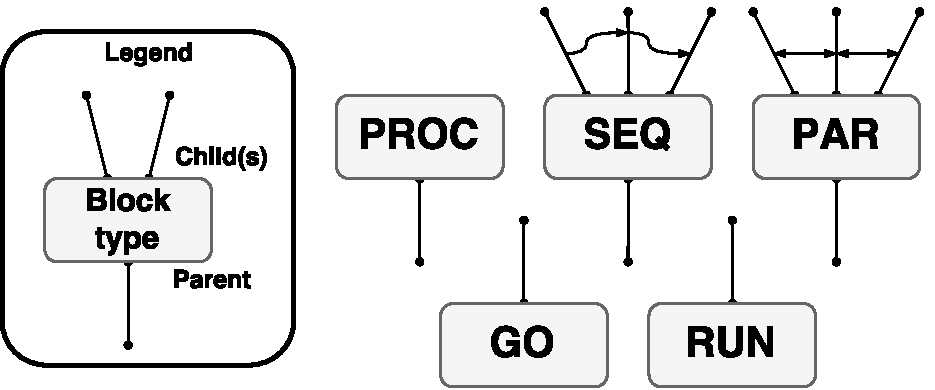
\includegraphics[width=0.8\linewidth]{fig/csp}
    \caption{Building blocks for composite processes}
    \label{fig:composite_blocks}
\end{figure}

\FloatBarrier

The combination of these building blocks can form any type of composite process. What is important to take away from this is that a composite process must \underline{\smash{always}} contain one, and only one, root node of either \texttt{GO} or \texttt{RUN}, and \underline{\smash{always}} contain one\hyp{}or\hyp{}more leaf nodes of \texttt{PROC}. 

Branch nodes, \texttt{SEQ} or \texttt{PAR}, with only one child does not alter the composite process behaviour. This becomes evident when we define a composite process of only one \texttt{PROC}, where it does not matter if multiple branch nodes of \texttt{SEQ} or \texttt{PAR} are present. This means branch nodes with one child are optional and redundant. See Figure \ref{fig:composite_axiom} for reference. 

\FloatBarrier

\begin{figure}[h]
    \centering
    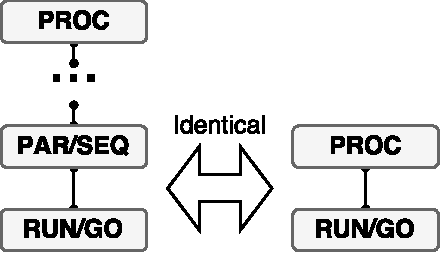
\includegraphics[width=0.5\linewidth]{fig/composite_axiom}
    \caption{Redundancy of branch nodes with one child}
    \label{fig:composite_axiom}
\end{figure}

\FloatBarrier

A composite process with a single process does not need a branch node, however a composite process with two\hyp{}or\hyp{}more \texttt{PROC} \underline{cannot} be expressed without at least one\hyp{}or\hyp{}more branch nodes.

\subsection{Composite Process Execution}

When a process defines a composite process, the run\hyp{}time system parses the FIXME definitions and creates a temporary composite process tree. The running process is marked as the root process of the composite process tree. The composite process tree is then traversed by the run\hyp{}time system, described by the pesudo\hyp{}code in Listing \ref{lst:algo_composite_process_tree_traversal}.

%\begin{enumerate}[topsep=0em,itemsep=-1em,partopsep=1em,parsep=1em]
%\label{algo:composite_process_tree_traversal}
%    \item \label{traversal_start} Given a node, initialized with child node of root node.
%    \item If the node is a \texttt{PROC} block
%    \begin{enumerate}[topsep=-1em,itemsep=-1em,partopsep=-1em,parsep=1em]
%        \item Create the process and add it to the ready queue of a scheduler.
%        \item Stop traversing.
%    \end{enumerate}
%    \item If the node is a \texttt{SEQ} block with positive non\hyp{}zero N childs
%    \begin{enumerate}[topsep=-1em,itemsep=-1em,partopsep=-1em,parsep=1em]
%        \item Register number of childs left on this node to N.
%        \item Traverse to the leftmost child node.
%        \item Goto \ref{traversal_start}.
%    \end{enumerate}
%    \item If the node is a \texttt{PAR} block with positive non\hyp{}zero N childs
%    \begin{enumerate}[topsep=-1em,itemsep=-1em,partopsep=-1em,parsep=1em]
%        \item Register number of childs left on this node to N.
%        \item Traverse to all child nodes.
%        \item For all child nodes, goto \ref{traversal_start}.
%    \end{enumerate}
%    \item Return Error.
%\end{enumerate}

\begin{lstlisting}[style=CustomC,caption={Pseudo code for the composite process tree traversal algorithm},label={lst:algo_composite_process_tree_traversal}]
// Called with the child node of the root node
int traversal(Node node) {
	switch (node.type) {
	case PROC:
		process = create_process(node.fxn_and_args);
		reschedule(process);
		return Ok;
	case SEQ: // fallthrough
	case PAR:
	    if (node.num_childs < 1) return Error;
	    if (node.num_childs == 1) {
	        node.parent.this_node = node.child;
	        return traversal(node.child);
	    }
		node.childs_left = node.num_childs;
		if (node.type == SEQ) {
			return traversal(node.leftmost_child);
		} else {
		    for_each(child in node.childs) {
		    	if (traversal(child) != Ok) return Error;
		    }
		    return Ok;
		}
	}
	return Error;
}
\end{lstlisting}

After the composite process tree is traversed, all initial processes are created and added to the ready queue in the scheduler. One thing to remark about the algorithm is that process creation is lazily evaluated \citep{lazyevaluation}, which means the processes are created when needed. This is entirely the consequence of the \texttt{SEQ} block behaviour. 
Now, whether the execution type is specified to be asynchronous or synchronous, the root process continues execution or transitions process state from \textit{Ready} to \textit{Wait}, respectively. For the synchronous case, the root node transitions from \textit{Wait} to \textit{Ready} when all \texttt{PROC} in the composite process tree has ended. 

However, one also has consider the how the execution order of the composite process tree behaves when a \texttt{PROC} ends. The pseduo\hyp{}code in Listing \ref{lst:algo_composite_process_tree_proc_ended} how this is processed by the run\hyp{}time system.

%\begin{enumerate}[topsep=0em,itemsep=-1em,partopsep=1em,parsep=1em]
%\label{algo:composite_process_proc_end}
%    \item \label{procend_start} Given a node, initialized with the ended \texttt{PROC}.
%    \item If the node is a \texttt{GO} block
%    \begin{enumerate}[topsep=-1em,itemsep=-1em,partopsep=-1em,parsep=1em]
%        \item Return Ok.
%    \end{enumerate}
%    \item If the node is a \texttt{RUN} block
%    \begin{enumerate}[topsep=-1em,itemsep=-1em,partopsep=-1em,parsep=1em]
%        \item Reschedule the root process.
%        \item Return Ok.
%    \end{enumerate}
%    \item If the node is a \texttt{PROC} block
%    \begin{enumerate}[topsep=-1em,itemsep=-1em,partopsep=-1em,parsep=1em]
%        \item Traverse to the parent node.
%        \item Goto \ref{procend_start}.
%    \end{enumerate}
%    \item If the node is a \texttt{SEQ} block with registered positive non\hyp{}zero M childs left
%    \begin{enumerate}[topsep=-1em,itemsep=-1em,partopsep=-1em,parsep=1em]
%        \item Decrement M.
%        \item If M is zero
%        \begin{enumerate}[topsep=-1em,itemsep=-1em,partopsep=-1em,parsep=1em]
%            \item Traverse to the parent node.
%            \item Goto \ref{procend_start}.
%        \end{enumerate}
%        \item Apply the traversal algorithm to the child node right to the returning child node.
%        \item Return the return value of the traversal algorithm.
%    \end{enumerate}
%    \item If the node is a \texttt{PAR} block with registered positive non\hyp{}zero M childs left
%    \begin{enumerate}[topsep=-1em,itemsep=-1em,partopsep=-1em,parsep=1em]
%        \item Decrement M.
%        \item If M is zero
%        \begin{enumerate}[topsep=-1em,itemsep=-1em,partopsep=-1em,parsep=1em]
%            \item Traverse to the parent node.
%            \item Goto \ref{procend_start}.
%        \end{enumerate}
%        \item Return Ok.
%    \end{enumerate}
%    \item Return Error.
%\end{enumerate}

\begin{lstlisting}[style=CustomC,caption={Pseudo code for the composite process tree \texttt{PROC} ended algorithm},label={lst:algo_composite_process_tree_proc_ended}]
// Called with the ended PROC
int proc_end(Node node) {
	while (true) {
		switch (node.type) {
		case RUN:                           
			reschedule(node.root_process);  @\label{line:root_process_start}@
		case GO: // fallthrough
			return Ok;
		case PROC:
			node = node.parent;
			continue;
		case SEQ: // fallthrough    @\label{line:backtrack_start}@
		case PAR:
			if (--node.childs_left == 0) {
				node = node.parent;
				continue;
			}
			return (node.type == SEQ)
				? traversal(node.next_in_sequence)
				: Ok;               @\label{line:backtrack_stop}@
		}
		return Error;
	}
}
\end{lstlisting}

The algorithm starts at the ended \texttt{PROC} and backtracks down the tree until hitting either the root node or a branch node with remaining childs left. Whenever entering a branch node, decrement the number of childs left for the given branch node. A resulting value of zero indicates all childs of the given branch has ended, and backtrack to the parent of the branch node. A resulting non\hyp{}zero value indicates there are still childs of the given branch node that are unfinished. For a \texttt{PAR} block this means the remaining childs are dispatched and will invoke the algorithm when ended. For a \texttt{SEQ} block this means there is a sequence of one\hyp{}or\hyp{}more childs remaining to be dispatched, for which the travel algorithm is called on the next child in the sequence. This is described on the lines \ref{line:backtrack_start} to \ref{line:backtrack_stop} in Listing \ref{lst:algo_composite_process_tree_proc_ended}.

The rescheduling of the root process in a synchronous composite process is described on line \ref{line:root_process_start} in Listing \ref{lst:algo_composite_process_tree_proc_ended}.

\section{Channels}

Channels forms the means of interprocess communication and synchronization, following the message passing model. There are mainly three aspects of channel design that must be considered, namely synchronous or asynchronous communication, channel disjointness, and type\hyp{}safe data transfer. 

\subsection{Synchronous and Unbuffered, or Asynchronous and Buffered}

Coming from the CSP model, channels are implemented as unbuffered and synchronous, and are sometimes called a synchronous rendezvous. This is used as a one\hyp{}way transfer of data between a receiver and a sender. Both the receiver and sender must be available at the channel for the transfer to occur. If one of the ends are not present, the other end must wait until both ends are ``ready''.

This channel design follows the CSP model, being unbuffered and synchronous.

\subsection{Channel Disjointness}

Some channels have a notion of disjointness \citep[see][chapter 3.3.1]{xc}, setting restrictions on how many processes are allowed to use a channel, and how many unique senders or receivers a channel can have. These designs are often denoted as a one\hyp{}to\hyp{}one, any\hyp{}to\hyp{}one, one\hyp{}to\hyp{}any, or any\hyp{}to\hyp{}any channels, following the \textit{\#Senders}\hyp{}to\hyp{}\textit{\#Receivers} scheme.

Creating four version of the channel design, one for each of the four combinations of \textit{one} and \textit{any}, might turn out to be a flexible approach. This allows the programmer to handpick the channel type for certain use cases, i.e.  one\hyp{}to\hyp{}any for multiple readers and one writer, etc.. 

One might argue ``Why not just have a any\hyp{}to\hyp{}any design, and cover all use cases?''. Enforcing disjointness increases the expressiveness of the abstraction, allowing the programmer to create more correct programs that reflects a truer behaviour of the system. As well, this also gives the implementation some assumptions allowing better optimizations for each design. 

This however has to be taken in consideration during implementation. If disjointness proves to be too difficult and/or impractical to implement, an any\hyp{}to\hyp{}any channel will suffice. 

\subsection{Type\hyp{}Safety}

Channels are also used to transfer data between processes. Type errors can be an issue in a data transfer, where the type of data sent over a channel does not match the type of data expected to be received. 

An example can be a sender and a receiver on a channel with no type\hyp{}safety. Sender sends a message of type A, which has a 4 byte size representation. Receiver B expects to receive a message of type B, which has a 2 byte size representation, and allocates the appropriate memory. When the transfer of data occurs, the channel writes the 4 bytes of data to the memory allocated only for 2 bytes. 2 bytes are written past the allocated memory, and memory corruption has occurred. See illustration in Figure \ref{fig:type_error} for reference. This illustrates the dangers of not enforcing type\hyp{}safety on channels. 

\FloatBarrier

\begin{figure}[h]
    \centering
    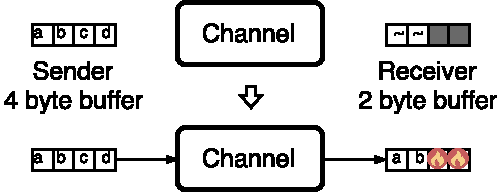
\includegraphics[width=0.6\linewidth]{fig/type_error}
    \caption{Memory corruption from conflicting types between sender and receiver}
    \label{fig:type_error}
\end{figure}

\FloatBarrier

Type\hyp{}safe channels enforces only transfer of messages of only one type. This in turn enforces the sender and receiver to agree on the type of the message. This should be favorable, as type errors should be treated as bugs in a program. Channels should therefore be as type\hyp{}safe as possible.

C is however known for not being very type\hyp{}safe. The language enforces type\hyp{}safety to some degree, but is easily circumventable through type casting to pointer types. A common source of type errors in C programs are pointers casted from and to void pointers, \texttt{void*}. Void pointers are used for memory with an unspecified type, which are convenient for implementation of generic interfaces. This is most likely how channels will implement data transfer, being compatible with any type. Knowing this, complete type\hyp{}safe channels in C will be impossible without code bloat and breaking encapsulation\footnote{This is possible, but requires heavy use of macros and leaking implementation details to the programmer}. A compromise is size\hyp{}safe channels. Instead of ensuring the type matches, the size representation of the type must match on both sides. This should not require much overhead, and at least avoids memory corruption, illustrated in Figure \ref{fig:type_error}.

\subsection{Complete Design}

Summary of complete design, the channel is synchronous and unbuffered. Should support the four disjoint restriction schemes one\hyp{}to\hyp{}one, any\hyp{}to\hyp{}one, one\hyp{}to\hyp{}any, or any\hyp{}to\hyp{}any to the degree of what is possible, and enforces size\hyp{}safety on the data transfer.


\section{Alternation}




\section{Timers}



\section{Thread Specific Data}
\label{sec:thread_specific_data}




\section{Descheduling Points}




\section{API}




\section{Influences}



